% capitulo de implementación
\chapter{Diseño e Implementación}
En el siguiente capítulo se describen las etapas recorridas para llegar a la solución que propone este proyecto.
\section{Arquitectura de la solución}
El siguiente capitulo consta de las bases necesarias para realizar la solución, la que se compone de dos elementos principales. 
\begin{itemize}
\item Servidor: Encargado de recodificar (si es necesario) la fuente de audio o video y segmentarla para su distribución.
\item Cliente: Aplicación ejecutada en iOS, encargada de comunicarse al servidor para pedir el flujo de video y entregar información en twitter.
\end{itemize}
% poner figura aqui
La figura \ref{diagramaGral} presenta una idea general del sistema.\\

\begin{figure}[H]
	\centering
	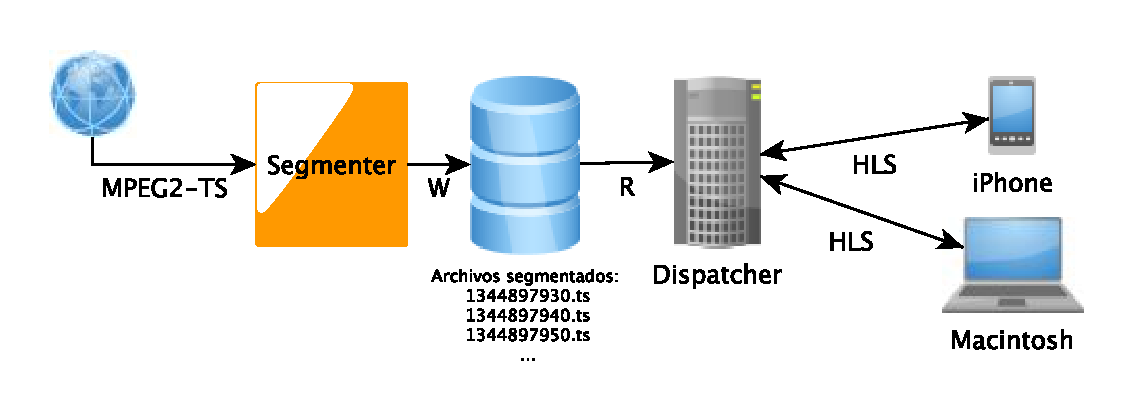
\includegraphics[scale=0.8]{imgs/diagrama_general.eps}
	\caption{Diagrama general de la solución}
	\label{diagramaGral}
\end{figure}

Respecto a los elementos principales, estos se componen de distintos modulos que serán explicados con más detalle a lo largo del capítulo. Del diagrama se explican de forma general:
\begin{itemize}
\item Segmenter: es una aplicacion que recibe como entrada un flujo de audio y/o video encapsulado en MPEG2-Transport Stream, para luego segmentar el contenido en archivos de menor duración, estos se guardan en el sistema de archivos del servidor.
\item Dispatcher: Este es un programa dedicado a recibir peticiones de los clientes, para entregar un flujo de video mediante el protocolo HTTP Live Streaming.
\item iPhone y Macintosh: Son los dispositivos clientes controlados por el usuario, en estos se realiza el intercambio de ordenes para recibir el flujo de video que se quiere ver.
\end{itemize}

\subsection{Requerimiento Obligatorio}
% https://developer.apple.com/news/index.php?id=02162010a
	El protocolo utilizado para entregar el contenido audiovisual es \textit{HTTP Live Streaming} (HLS), el que se eligió debido a requerimientos obligatorios designados por Apple para la distribución de contenidos multimedia para su sistema operativo iOS.\\
	
	En un anuncio realizado por Apple en su sitio web destinado a desarrolladores, indica como obligación que la entrega de contenido del tipo audio y/o video con una una duración mayor a 10 minutos debe utilizar necesariamente el protocolo \textit{HTTP Live Streaming} ya sea el enlace mediante WiFi o red celular. Además las aplicaciones deben incluir un flujo de datos (\textit{stream}) de baja calidad con una cadencia de datos no superior a 64 Kilobits/segundo, de manera que estas aplicaciones mantengan fluidez de contenido a pesar de encontrarse en condiciones desfavorables en la red.
	
	En caso de no seguir esta indicación, el desarrollador arriesga que su aplicación no sea admitida en la plataforma principal para la distribución de aplicaciones: iTunes Store.

	Considerando que este trabajo de memoria busca incorporar a los dispositivos iOS como consumidores del contenido multimedia utilizando saltos temporales (TimeShift), se debió diseñar la solucion alrededor de este protocolo.

%en resumen un acercamiento a como funciona la cosa

%\part{Primera parte}
\section{Protocolo HTTP Live Stream}
% https://developer.apple.com/resources/http-streaming/
% http://en.wikipedia.org/wiki/HTTP_Live_Streaming
% http://en.wikipedia.org/wiki/Progressive_download
% http://en.wikipedia.org/wiki/HyperText_Transfer_Protocol

El protocolo \textit{HTTP Live Streaming} o HLS (abreviado), es un protocolo desarrollado por Apple Inc. para la distribución de multimedia a través de redes de computadores, de manera que el usuario consume el producto a medida que se descarga, es decir de forma continua.\\

Su carácteristica principal es la utilización del protocolo para transferencias de hipertexto, HTTP (\textit{hypertext transfer protocol}) por sus siglas en inglés. Si bien HTTP se diseño originalmente para la \textit{\textbf{World Wide Web}} como vía de entrega del texto en formato HTML, este se puede utilizar para distribuir datos de otros formatos codificados para habilitar su distribución.\\

HLS funciona entregando el contenido de forma segmentada al cliente, el cual tiene la responsabilidad de manejar la lógica de cambio de segmentos. Para distribuir el contenido se codifica la fuente de audio y/o video en varios archivos de corta duración, recomendandose 10 segundos \cite{bib:tensec-targetduration}, y que pueden o no tener el mismo bitrate. Estos pequeños archivos se ordenan en una lista de reproducción de formato .M3U8 que se entrega al reproductor del cliente. \\

También existe una variante donde la lista de reproducción contiene referencias a otras listas de reproducción con otras variantes de flujos de datos. \\

% http://www.streamingmedia.com/Articles/Editorial/What-Is-.../What-is-HLS-(HTTP-Live-Streaming)-78221.aspx
% In the Apple App Store, if you produce an app that delivers video longer then ten minutes or greater than 5MB of data, you must use  HTTP Live Streaming, and provide at least one stream at 64Kbps or lower bandwidth. Any streaming publisher targeting iOS devices via a website or app should know the basics of HLS and how it’s implemented.
	\subsection{Especificación}
		El protocolo HLS consiste en ordenar la entrega de archivos discretos a través de HTTP.
		El procedimiento general consiste en segmentar el contenido multimedia (audio y/o video) en pequeños archivos de manera que a través de un servidor web regular el cliente pueda descargar y unir los segmentos para verlos de manera continua. Esta forma de entregar el contenido puede ser utilizada para contenido pre-grabado o en vivo, difiriendo levemente en el componente encargado de ordenar los segmentos.\\
		
\begin{figure}[H]
	\centering
	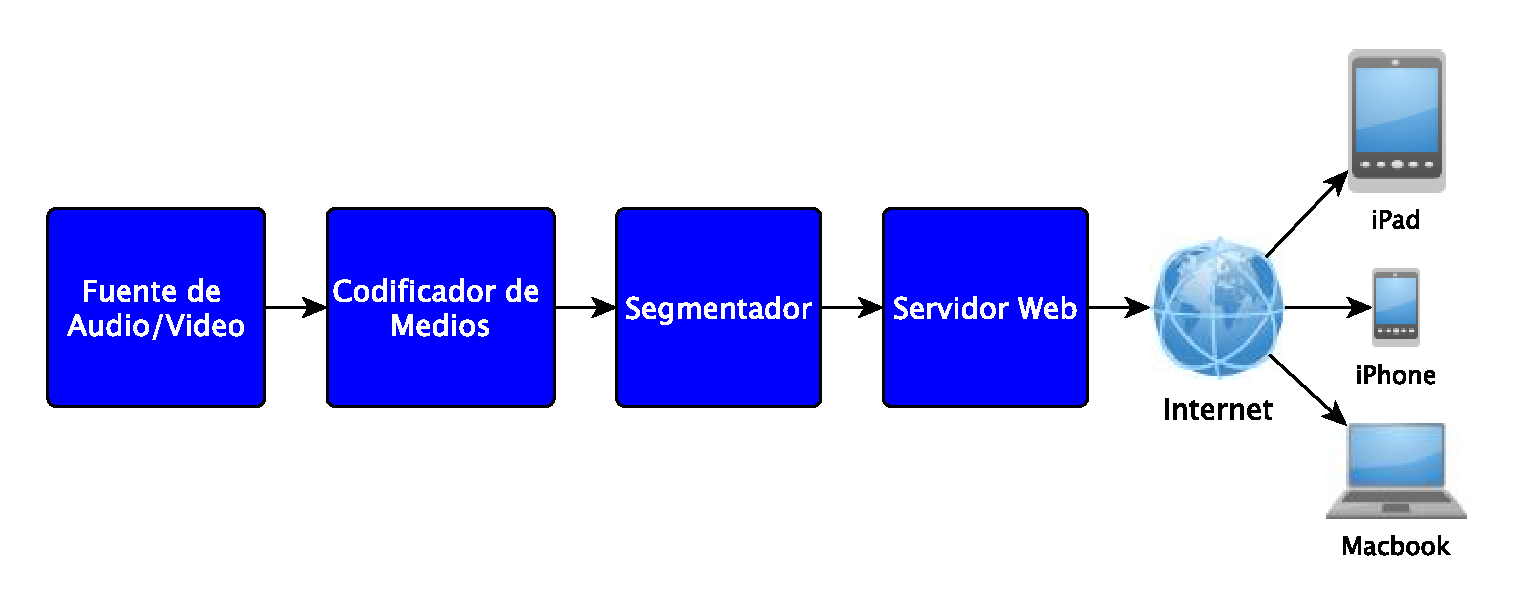
\includegraphics[scale=0.5]{imgs/HLS_diagram_wwdc2010.eps}
	\caption{Flujo de trabajo de HTTP Live Streaming}	
	\label{diagramaHLSwwdc2010}
\end{figure}		
		La figura \ref{diagramaHLSwwdc2010} presenta un ejemplo de distribucion de multimedia a través de HTTP Live Streaming.\\
		
En primera instancia se debe obtener contenido multimedia ya sea en un archivo fijo o flujo de datos, este contenido debe ser codificado para que sea compatible con los dispositivos que corren iOS, generalmente por recomendación de Apple se deben utilizar los codec de video h.264 y de audio AAC (advanced audio coding). El empaquetado de este contenido ya codificado debe ser entregado a una aplicación encargada de segmentarlo en pequeños archivos. \\

	El flujo de transporte a utilizar es MPEG2-TS (MPEG2 Transport Stream), el resultado de la aplicación segmentadora es guardado en el sistema de archivos donde reside el servidor web (o una ubicación accesible) de manera que al recibir requerimientos de stream HLS, este pueda proveer una lista de reproducción en formato M3U8 que mantiene el orden de reproducción de los archivos.\\
	
Tomando en cuenta el funcionamiento del protocolo HLS, para distribuir el contenido multimedia generado en vivo se debe codificar y segmentar inmediatamente para que el servidor web pueda proveerlos. En el caso de que el contenido sea un gran archivo, la codificación y segmentación se realiza una sola vez.

\subsubsection{Lista de reproducción}
\label{TAG-SECTION}
La lista de reproducción en formato M3U8 es lo que se entrega al cliente, el cual puede ser una aplición iOS o el navegador web Safari desarrollado por Apple. Esta lista consiste en enlaces (URL) absolutos o relativos de los segmentos siguiendo el orden del contenido. Además se incluyen comentarios precedidos por el caracter \textbf{\#}, en el caso que un comentario utilice una palabra conocida del protocolo se le denomina entonces como marca (tag).
Las marcas primordiales para una trasmision a través de HLS son las siguientes:

\begin{prop}

\item \#EXTM3U: Corresponde a la primera marca que inicia una lista de reproducción, siempre debe estar al principio.

\item \#EXT-X-TARGETDURATION: Esta marca corresponde a la mayor duración que puede poseer cualquier segmento, es decir los segmentos enumerados en la lista no pasarán del tiempo especificado por esta marca.
Además este valor indica al cliente cada cuanto tiempo debe realizar una petición al servidor web por la lista.
\label{TAG-targetduration}

\item \label{TAG-mediasequence} \#EXT-X-MEDIASEQUENCE: Corresponde a la secuencia o versión de la lista de reproducción segun los segmentos que se incluyen dentro de ella. Este valor se representa por un número entero y debe ser consecuente a los cambios en el contenido, es decir, si se agregan nuevos segmentos el valor de la secuencia debe aumentar, de esta forma el cliente puede saber que el flujo de contenido se está actualizando.


\item \label{TAG-extinfint} \#EXTINF: Esta marca indica la duración del segmento que se encuentra junto a él. Su valor está indicado por un número entero que representa los segundos.\\
\end{prop}

\begin{figure}[H]
	\centering
	\begin{lstlisting}
	#EXTM3U
	#EXT-X-TARGETDURATION:10
	#EXT-X-MEDIA-SEQUENCE:1
	#EXTINF:10,
	http://media.ejemplo.com/segmento0.ts
	#EXTINF:10,
	http://media.ejemplo.com/segmento1.ts
	#EXTINF:10,
	http://media.ejemplo.com/segmento2.ts
	#EXT-X-ENDLIST
	\end{lstlisting}
	\caption{Lista de reproducción del tipo Video-on-Demand}
	\label{ejemploM3U8}	
\end{figure}			

El ejemplo visto en la figura \ref{ejemploM3U8} destaca una marca extra: \#EXT-X-ENDLIST, la cual indica al cliente que la lista de reproducción está completa y no necesita ser actualizada. Esta marca toma gran importancia al definir un flujo de medios ``en vivo'' ya que al estar ausente el cliente pedirá una nueva versión de la lista de reproducción que incluya nuevos segmentos, el tiempo que indica la actualización depende de la marca \ref{TAG-targetduration} previamente explicada.\\

En el caso de contenido en vivo, la lista de reproducción toma el rol de \textbf{ventana de reproducción}  como la lista se actualiza con nuevos segmentos cada intervalo de \ref{TAG-targetduration} se evita un archivo de gran tamaño al eliminar segmentos ya pasados.

Cabe destacar que la marca \ref{TAG-mediasequence} debe mantener consistencia con los nuevos segmentos, es decir si la lista elimina un segmento pasado y agrega uno nuevo, el numero de secuencia debe aumentar su valor.\\

Para efectos de la solución de este trabajo de memoria el modo de flujo de datos a utilizar con HLS es del tipo ``en vivo''.
\subsubsection{Segmentos}
Los segmentos consisten en video codificado con h.264 y audio en AAC. Apple indica que también es compatible MP3, sin embargo se decidió por AAC debido a su mayor compresión de audio y permitiendo así transmitir un mejor sonido a menor ancho de banda. En el sitio web \cite{apple-hlsencoding} se indican los perfiles recomendados para codificar el contenido a trasmitir con HTTP Live Streaming, para mantener compatibilidad con clientes que estén adoptando el protocolo se utilizó  
\begin{itemize}
\item Video: H.264 Baseline Profile Level 3.0, resolución 480x320 y tasa de fotogramas 29.97

\item Audio: AAC-LC, 48 kHz, stereo.

\end{itemize}

La duración de los segmentos se limitó a 10 segundos por recomendación del mismo documento técnico (TN224 \cite{apple-hlsencoding}), donde indica explícitamente: \textit{\textquotedblleft Use 10 second Target Durations"}, utilice 10 segundos de duración de objetivos.

% El contenedor de los medios es MPEG2-TS según la especificación del protocolo HLS. Las indicaciones de Apple sugieren tener cuidado con el overhead.
		% mostrar figura de playlist, explicacion rapida de como funciona hls
\subsubsection{Borrador IETF}
Apple Inc. es la compañía desarrolladora de este protocolo. Para masificar su uso en dispositivos móviles ha dispuesto un borrador como propuesta para la estandarización del protocolo según la \textbf{IETF} (\textit{Internet Engineering Task Force}).
Debido a la popularidad de los dispositivos móviles con iOS, empresas importantes en el desarrollo de tecnologias para difusión de medios han adoptado el protocolo HLS como salida de productos dedicados a la codificación y/o transmisión de multimedia. Ejemplos como Adobe Systems con su producto Adobe Flash Media Server, Wowza Media Systems con Wowza Media Server y VideoLan con VLC Media Player demuestran que la investigación realizada por los ingenieros de Apple Inc. Roger Pantos y William May, Jr, han sentado las bases para cualquier desarrollo asociado con el protocolo.\\

Para el desarrollo de esta memoria se han implementado aplicaciones y scripts que utilizan las herramientas e instrucciones detalladas en el documento borrador. A lo largo de la investigación los ingenieros desarrolladores incorporaron caracteristicas nuevas que fueron aprovechadas para lograr el cometido de esta memoria.\\

En sitio web \cite{apple-draftpantos} se puede revisar detalladamente el documento completo. En esta sección se describen las marcas utilizadas aparte de las ya descritas en \ref{TAG-SECTION}:

\begin{itemize}
\item \#EXT-X-VERSION: Corresponde a la versión de la lista de reproducción, se utiliza para diferenciar distintos streams con protocolo HLS según las caracteristicas que se van incorporando. Para el trabajo de esta memoria se utiliza la versión 3 del protocolo.

\item \#EXTINF: Si bien ya se ha descrito esta marca en \ref{TAG-extinfint}, a partir de la versión 3 del protocolo HLS, la marca \textbf{EXTINF} permite valores flotantes para mejorar por parte del cliente la exactitud en el seguimiento del tiempo de reproducción. 

\item \#EXT-X-PROGRAM-DATE-TIME: Marca correspondiente a la fecha asociada al primer segmento de datos que aparece en la lista de reproducción. La fecha se especifica utilizando el estandar ISO 8601, y opcionalmente se puede incluir zona horaria. Un ejemplo del formato sería:

\begin{lstlisting}
#EXT-X-PROGRAM-DATE-TIME:2011-12-18T14:54:23-04:00
\end{lstlisting}

Correspondiente al día 18 de diciembre de 2011, a las 14:54:23 en la zona horaria GMT-4.

\end{itemize}
		% aqui detallar los mensajes de la playlist utilizados
		%		http://tools.ietf.org/html/draft-pantos-http-live-streaming-08
\subsubsection{Lista de Variantes}
Más allá de la lista de reproducción con segmentos, el protocolo HLS posee caracteristicas anexas para mejorar la experiencia del usuario.
Una de las caracteristicas a utilizar y que también es requisito para que las aplicaciones con multimedia remota puedan ser aprobada en la App Store es la necesidad de una variante del stream por donde se transmita solamente el audio.\\

Para solucionar este requerimiento y cumpliri la obligación se utiliza una lista de variantes, la cual consiste en una lista de reproducción que incluye en su interior URLs hacia listas de reproducción normales ya explicadas anteriormente, la diferencia cae en que cada lista de reproducción tiene asociado un ancho de banda límite, de manera que el cliente pueda cambiar de stream dentro de la reproducción sin que el usuario note el cambio en la reproducción, exceptuando la calidad del audio o del video.\\

Se utiliza la marca \textbf{\#EXT-X-STREAM-INF} para asociar cada una de las variantes del stream a cierto ancho de banda, además cada una posee los siguientes atributos:

\begin{itemize}

\item \textbf{PROGRAM-ID}: Corresponde a un valor numérico entero, tiene como fin identificar una presentación en particular dentro de la ventana de transmisión de la lista de reproducción. Una lista de variantes puede contener multiples sublistas con distintos programas de forma que este atributo asocia las distintas variantes para una transmisión en particular, entiendase por show o evento a transmitir. Esta caracteristica puede ser opcional.

\item \textbf{BANDWIDTH}: Este atributo obligatorio representa el valor entero de los bits por segundo, como requisito principal el valor debe ser la cota mayor de la tasa de bits promedio de los segmentos (incluyendo el overhead del contenedor) que aparecen o aparecerán en la lista de reproducción. 

\end{itemize}

El enlace a las sublistas de variantes del stream pueden ser del tipo relativo o absoluto. Como requisito cada variante del stream debe poseer el mismo valor en segundos de Target Duration \ref{TAG-targetduration}.

\begin{figure}[H]
	\centering
	\begin{lstlisting}
	#EXTM3U
	#EXT-X-STREAM-INF:PROGRAM-ID=1,BANDWIDTH=110000
	varianteA/prog_index.m3u8
	
	#EXT-X-STREAM-INF:PROGRAM-ID=1,BANDWIDTH=200000
	varianteB/prog_index.m3u8

	#EXT-X-STREAM-INF:PROGRAM-ID=1,BANDWIDTH=350000
	varianteC/prog_index.m3u8

	#EXT-X-STREAM-INF:PROGRAM-ID=1,BANDWIDTH=550000
	varianteD/prog_index.m3u8

	#EXT-X-STREAM-INF:PROGRAM-ID=1,BANDWIDTH=900000
	varianteD/prog_index.m3u8

	\end{lstlisting}
	\caption{Lista de variantes para HTTP Live Streaming}
	\label{ejemploVariantPLS}	
\end{figure}	

En la figura \ref{ejemploVariantPLS} se observan tres variantes asociadas al mismo PROGRAM-ID de valor 1. La diferencia entre ellas recae en el ancho de banda límite.\\

Por defecto la primera variante será la utilizada para comenzar la transmisión, y además se utilizará para revisar la calidad del enlace, si la velocidad de descarga de los segmentos da como resultado un mayor ancho de banda, el cliente cambiará a la variante con el mayor valor que pueda cubrir este calculo de ancho de banda.\\

En el caso que exista por distintos motivos una caida en la calidad del enlace, la baja de velocidad de descarga debe ser alertada por el cliente de forma que pueda cambiar la variante en reproducción por otra asociada a un menor ancho de banda. Estos cambios deben ocurrir de manera automatica de modo que al usuario no se le vea afectado el flujo que está consumiendo.\\

Tomando en cuenta este comportamiento, se debe considerar al armar la lista de variantes según el tipo de enlace que utilizarán sus clientes. Por ejemplo si tiene identificado que sus clientes se conectarán al servidor mediante WiFi es preferible que la lista de variantes tenga como primer elemento la variante de 550000 Kbps y en caso de que sus clientes se conecten al servidor mediante red celular, es preferible presentar como primer variante la de 110000 Kbps.
	De esta forma el cliente reproducirá inmediatamente un stream acorde a su enlace. \\
	
En el ejemplo de la figura \ref{ejemploVariantPLS} a través de red celular el cliente podrá reproducir el contenido rápidamente con velocidades EDGE, y si el enlace lo permite podrá cambiar a una mejor variante. En caso de que el cliente se conecte mediante WiFi, cargará el enlace de menor ancho de banda para realizar pruebas e inmediatamente descartarlo por uno de mejor calidad que satisfaga sus requerimientos.

% recomendaciones de apple, bitrates y bw



% caracteristicas bacanes de hls, detallar lo que se puede hacer más aun
	\subsection{Herramientas dispuestas por Apple}
	Apple Inc. como desarrollador y promotor de esta tecnología ha dispuesto para los desarrolladores un set de aplicaciones de línea de comandos para la creación de transmisiones con HTTP Live Streaming.
		\subsubsection{MediaFile Segmenter}
Esta aplicación tiene como funcion multiplexar el contenido multimedia del archivo en un flujo de transporte MPEG2 (MPEG2-TS) y dividirlo en una serie de pequeños archivos de aproximadamente la misma duración. La aplicación también crea una lista de reproducción con referencias a los archivos del tipo Video en demanda (VOD).

		\subsubsection{MediaStream Segmenter}
Al igual que MediaFile Segmenter, esta herramienta segmenta el contenido multimedia en varios archivos, sin embargo toma como entrada un flujo de transporte MPEG2 a través de un enlace UDP [dirección:puerto] o también puede hacerlo a través de la entrada estandar (stdin). De igual forma que \textit{mediafilesegmenter} esta aplicación genera una lista de reproducción en formato \textbf{m3u8}.\\

Como recibe de entrada un flujo de datos, permite generar listas de reproducción en vivo, generando segmentos mientras se reciben y actualizando la lista de reproducción con las referencias. Este tipo de flujo de medios es recomendable para difusión contínua, permitiendo además eliminar los segmentos que ya expiraron en la ventana de transmisión.

		\subsubsection{Variant Playlist Creator}
		Esta aplicación se utiliza en conjunto con MediaFile Segmenter para crear una lista de variantes a partir de multiples streams del tipo VOD. Esto se realiza indicando la opcion en MediaFile Segmenter \textit{--generate-variant-plist} que genera un archivo property list (XML) por cada variante del stream, estos archivos se entregan junto a las listas de reproducción para obtener la lista de variante.
			
		\subsubsection{MediaStream Validator}		
		Esta herramienta simula una sesión HLS y verifica que las listas de variantes y reproducción junto a los segmentos cumplen la especificación HTTP Live Streaming. Si se encuentra algún problema en las pruebas de reproducción, se entrega un informe para diagnostico.
		
	\subsection{Ejemplo de transmisión}

Con las herramientas provistas por Apple, se procedió a realizar una transmisión en vivo de prueba, codificando una pelicula ya comprimida en audio AAC y video h.264, los codificadores especificados como compatibles con iOS. Para generar un Stream de video UDP se utilizó la aplicación \textbf{VLC.app} de VideoLan, la cual permite la encapsulación del contenido en MPEG2-TS y su difusión a la misma máquina por UDP utilizando la dirección por defecto \textbf{udp://localhost:1234}. Para realizar esta transimisión se utiliza el \textit{asistente de emisión/transcodificación}.\\

\begin{figure}[H]
	\centering
	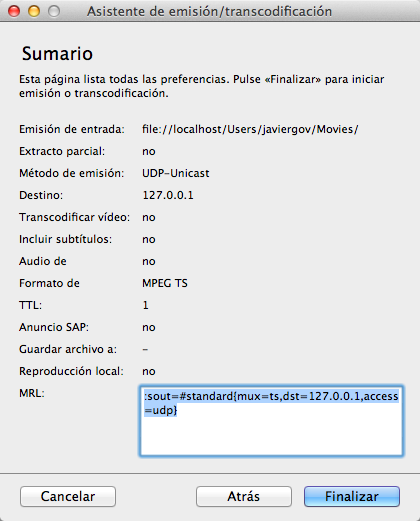
\includegraphics[scale=0.5]{imgs/vlc_transmission.png}
	\caption{Ajustes de la aplicación VLC.app para transmisión de película a través de UDP.}
	\label{vlc_transmission}	
\end{figure}


Considerando las herramientas y el escenario del contenido, la más indicada para transmitir a través de HLS es MediaStream Segmenter ya que puede tomar como entrada el flujo de datos emitidos por UDP y luego entregar su salida a un servidor web Apache que provea a través de internet. De esta forma clientes del tipo iPhone, iPad o Macintosh pueden acceder al contenido multimedia.\\

En la figura \ref{vlc_transmission} se puede observar que la emisión se ha realizado a una ip en específico utilizando el flujo de transporte MPEG2-TS. Este stream se entrega al \textbf{mediastreamsegmenter} con los siguientes parámetros en la línea de comandos.

 \begin{lstlisting}
	mediastreamsegmenter -s 7 -t 11 -D -i ejemplo.m3u8 
	-f ~/Sites/hlsexample 127.0.0.1:1234
\end{lstlisting}

Estos parámetros indican a mediastreamsegmenter que para el ejemplo se genere una lista de reproducción con una ventana de transmisión de \textbf{7} segmentos (\textbf{-s}), los cuales tienen \textbf{11} segundos de duración (\textbf{-t}), además se le indica que los segmentos ya caducados deben ser eliminados (\textbf{-D}). \\

La lista de reproducción lleva el nombre \textit{ejemplo.m3u8} (\textbf{-i}) y los archivos resultantes se deben guardar en el directorio con ruta \textit{$\sim$/Sites/hlsexample} (\textbf{-f}). Por ultimo se indica que la emisión UDP se halla en la dirección ip y puerto: \textit{127.0.0.1:1234}.\\

El resultado de esto es un stream HLS al cual se puede acceder mediante un servidor web como por ejemplo Apache. En caso de este ejemplo los archivos se ubican en el subdirectorio \textit{hlsexample} del directorio asignado a Apache del usuario, para acceder al stream se utilizó un player HTML5 en el archivo \textit{index.html} ubicado junto al resto.

 \begin{lstlisting}
	<html>
	<head></head>
	<body>
		<video src="ejemplo.m3u8" controls 
		autoplay height="360" width="640">
		</video>
	</body>
</html>\end{lstlisting}

Nótese que la fuente al video es la lista de reproducción generada por \textbf{mediastreamsegmenter}, la cual se encuentra en constante actualización mientras la transmisión se lleva a cabo.\\

Ya con el servidor web funcionando, la carga de esta página web permitirá la reproducción del stream en vivo mientras el navegador web sea compatible con el protocolo HTTP Live Streaming utilizando el player HTML5. En la actualidad los únicos navegadores compatibles son Safari y Mobile Safari, desarrollados por Apple.\\
\begin{figure}[H]
	\centering
	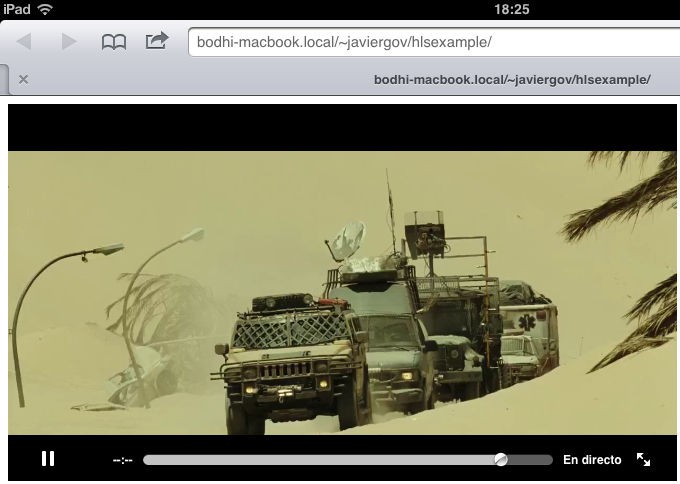
\includegraphics[scale=0.6]{imgs/ipad-hlsexample.png}
	\caption{Captura de pantalla de Mobile Safari en iPad}
	\label{ipad-hlsexample}	
\end{figure}

En la figura \ref{ipad-hlsexample} se puede observar que la reproducción del stream puede ser llevada a cabo por un dispositivo iOS accediendo a la página web creada.\\








	
%	explicar como se probó con resident evil y motorstorm
%	con variantes VOD y live
	
\section{Reproducción y Control de Stream de Video}

%	explicar resumido la estructura como se conecta el server y el cliente, con un  diagrama
	Este trabajo de memoria buscó entregar al usuario control de la linea temporal de un flujo de contenidos en vivo. Para realizar esto se ideó un sistema que intercambia marcas de tiempo entre el cliente y el servidor, de manera que aquel pueda definir desde qué punto el servidor debe crear una lista de reproducción en vivo. \\
	
	Para entregar esta información se utilizó como método de entrada parámetros en la url, que el cliente utiliza para conectarse. Además se puede mejorar la experiencia del usuario indicando al servidor el tipo de enlace que el cliente posee, es decir WiFi o red celular, y expandiendo aun más con un parámetro para definir el canal que se quiere ver, todo desde la misma aplicación.
	
	\subsection{Servidor HTTP}
	El servidor consiste en dos módulos: segmenter y dispatcher, este último depende de los archivos guardados por el segmentador, a su vez el segmentador recibe los datos a través de una emisión UDP o por la entrada estandar \textbf{stdin}.
		\subsubsection{Obtención del Stream}
%		la recepcion de un stream RTMP, codificacion con vlc o ffmpeg y generar un archivo o stream udp
El contenido puede ser obtenido de distintos tipos de fuentes pero este debe cumplir con la especificación de HTTP Live Streaming, es decir entregar al segmentador un flujo de datos codificados con perfiles compatibles con iOS y encapsulados en MPEG2-TS.
		\subsubsection{Sementación del Video}
		% el segmenter que corta su entrada en pedacitos de 10 seg, ademas guarda el tiempo inicial y el final de lo guardado, además se sacarán las fotitos.

El segmentador utilizado fue desarrollado por la empresa AltaVoz S.A. interesada en llevar a cabo el proyecto. Los motivos de este trabajo se deben a que las herramientas dispuestas por Apple funcionan sólamente en versiones recientes del sistema operativo Mac OS X. Al ver esta limitante la empresa se encarga de desarrollar un segmentador que se comporte de forma similar a \textbf{mediastreamsegmenter}, trozando el flujo de entrada en pequeños archivos de cierta duración.\\

 La gran diferencia con el uso de \textbf{mediastreamsegmenter} recalca en el almacenamiento de los archivos resultantes, estos se guardan sin ser eliminados para mantener un gran registro de las transmisiones, el nombre de cada segmento corresponde a la fecha y hora de la recepción de la emisión en formato Unix time (POSIX time) y con extensión \textbf{.ts}. Para mantener orden en el sistema de archivos los segmentos se guardan en subdirectorios por cada hora de contenido, el nombre de estos subdirectorios también llevan Unix time para su catalogación.\\

Una última caracteristica especial del segmentador es marcar el segmento más antiguo y el más reciente en dos archivos \textbf{\textit{start.txt}} y \textbf{\textit{last.txt}} respectivamente, de forma que el cliente pueda representar gráficamente al usuario la disponibilidad de contenido en el \textit{stream}.
		
		\subsubsection{Emisor de la lista de reproducción}
%		dispatcher que recibe epoch, el tipo (canal) y el bwPARAMETER del tipo de enlace Wifi o cellular		
El \textit{Playlist Dispatcher} consiste en un script \textbf{php} disponible en Internet gracias a un servidor web que trabaje con un módulo PHP, el script \textit{playlist dispatcher} debe recibir parámetros del cliente a través de la cadena de consulta (\textit{query string}) de la dirección URL. Los parámetros son los siguientes:

\begin{itemize}
	\item \textbf{t}: Corresponde a la marca de tiempo que el cliente quiere recibir, esta debe ser indicada con el formato Unix Time (POSIX time).
	\item \textbf{s}: Este parámetro indica al script cual contenido entregar a través del stream. Analogamente se puede considerar como el parámetro para definir cual canal de televisión el usuario quiere ver. El valor corresponde a una cadena de caracteres (\textit{string}).
	\item \textbf{c}: Este último parámetro corresponde al tipo de conexión con la cual el cliente está conectado a Internet, pueden ser dos valores, 1 para red celular y 0 para WiFi. Este parámetro se utiliza para optimizar la lista de variantes que entrega el script.
\end{itemize}
		
Con estos parámetros el playlist dispatcher retorna una lista de variantes con referencias a otro script que genera las listas de reproducción.
		
	\subsection{Cliente iOS}
%		descripcion general.
%		como se conecta al server, reachability, entrega a avplayer
Ha de entenderse por cliente una aplicación ejecutada sobre el sistema operativo \textbf{iOS}, su funcion consiste en mantener un enlace al servidor contactándose directamente con el playlist dispatcher y descargar los segmentos que éste le indique.\\

Además debe presentar en la pantalla del dispositivo el video, o reproducir el audio, según el tipo de stream. Para realizar esto se utilizan componentes de la interfaz de programación de aplicaciones (\textbf{API} - \textit{Application Programming Interface}). El cliente debe permitir al usuario controlar el contenido del stream con una interfaz gráfica simple y precisa.

		\subsubsection{Reproducción con AV Framework}
%		avplayer, playeritem, asset tracks		
Apple en su documentación indica referencias a componentes en iOS que son capaces de reproducir streams HLS, componentes de nivel más alto como por ejemplo un reproductor de video HTML5 anidado en una página web o la clase \textbf{MPMoviePlayerViewController} que pertenece a \textbf{Media Player Framework}, la que consiste en una pantalla que incorpora controles como barras deslizadoras para video y botones de control, facilitando de gran manera a los desarrolladores presentar contenidos multimedia. \\

Sin embargo como este trabajo buscó presentar una característica nueva a lo que es la reproducción de streams, se debió desarrollar un componente que se asemeje al estandar MPMoviePlayerViewController (fig. \ref{IMG-mpmpvc-example}) incluyendo la característica de control de contenido y compartir información a través de Twitter.\\

Uno de los componentes que significó una gran ayuda en el desarrollo del cliente es \textit{AV Foundation Framework}, la cual es una estructura de más bajo nivel que \textbf{Media Player Framework}. 
En la figura \ref{IMG-ios-tech-frameworks} se interpreta que los módulos de AV Foundation se encuentran bajo \textbf{UIKit}, el cual es la infraestructura para interfaces gráficas en iOS, por lo tanto al utilizar AV Foundation para reproducir contenido temporal del tipo audio o video es necesario implementar con los componentes de UIKit la salida gráfica para el usuario.\\

El motivo de utilizar AV Foundation, además de una interfaz gráfica personalizada, es la obtención de datos que las clases por defecto no entregan, datos que están relacionadas con el control personalizado de la reproducción.

% y que permite obtener mayor información de los componentes de un archivo o stream multimedia.

% imagen
\begin{figure}[H]
	\centering
	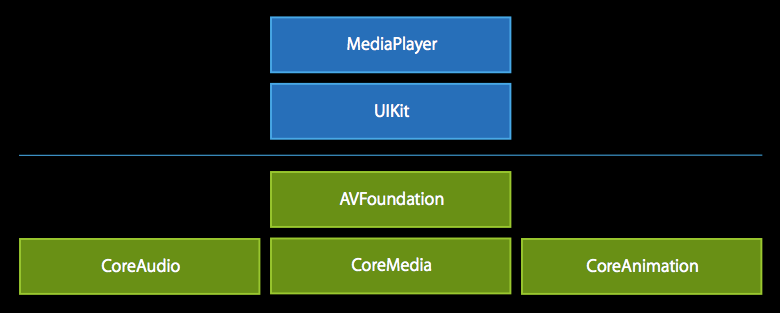
\includegraphics[scale=0.5]{imgs/ios-tech-frameworks.png}
	\caption{Infraestructuras tecnologicas para el manejo de multimedia en iOS}
	\label{IMG-ios-tech-frameworks}	
\end{figure}

% imagen
\begin{figure}[H]
	\centering
	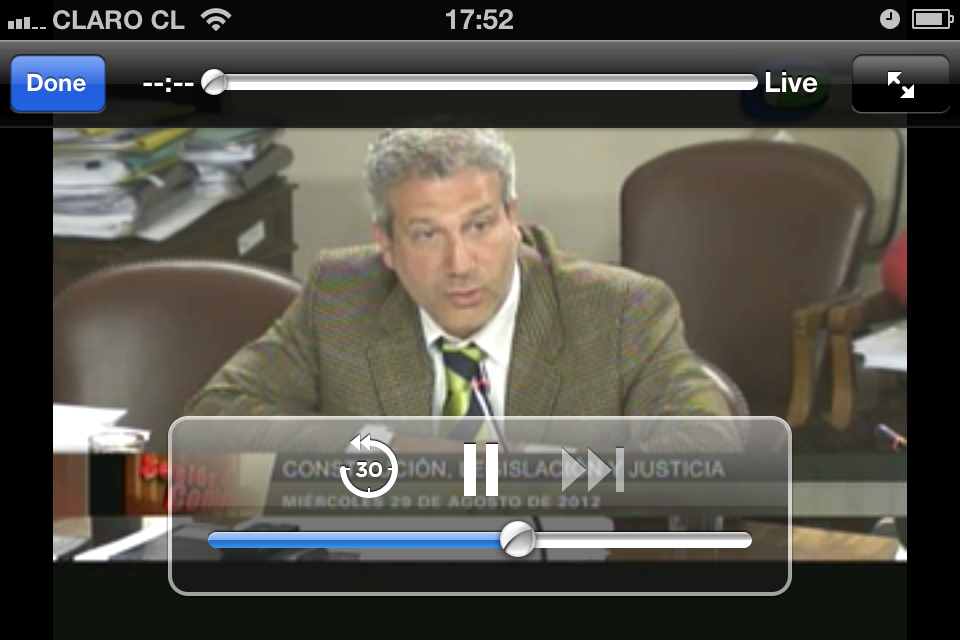
\includegraphics[scale=0.3]{imgs/mpmpvc-example.png}
	\caption{Aplicación reproduciendo stream HLS con MPMoviePlayerViewController}
	\label{IMG-mpmpvc-example}	
\end{figure}

		\subsubsection{Recopilación de datos del Stream}
%		kvo, notificaciones, periodic observers, la fecha y que se hace con ella
Utilizando observadores de notificaciones centralizadas (\textit{Notification Center} \cite{bib:ios-nsnotificationcenter}), observadores de cambio de valor (KVO - \textit{Key Value Observing} \cite{bib:kvo-guide}) y observadores periodicos (\textit{Periodic Observers} \cite{bib:avplayer-periodic}), es posible llevar un registro del contenido del stream, como tambien la mayoría de los cambios de estado del reproductor.\\

Para mantener de forma continua la información temporal del stream se han asociado a la instancia de la clase AVPlayer dedicada a la reproducción del stream entregado por URL, los siguientes datos.\\
% enumerar los datos obtenidos

\textbf{Revisión periódica}:

\begin{enumerate}
\item \textbf{Tiempo de reproducción}: Este se supervisa en un intervalo de 1/10 de segundo de forma que con esta razon de cambio la interfaz gráfica se actualice, se ajusta a  este valor de tiempo (100 ms) de forma que el usuario no identifique irregularidad en el temporizador y a la vez la carga en ciclos se ejución no afecte el desempeño de la máquina.
\item \textbf{Fecha asociada al stream}: Este valor es parte fundamental en el funcionamiento del stream con saltos en el tiempo, su origen se debe al tag asociado a la lista de reproducción del stream.
\label{observer-date}
% esto no está en la memoria, se hizo después para Janus.
%\item \textbf{Tasa de Bits}: Se obtiene el valor de la tasa de bits promedio del flujo de datos multimedia, para obtenerlo se deben separan los activos (AVAssets) del item (AVPlayerItem) en reproducción. 

\end{enumerate}

En el caso de la observación periódica de datos, esta se debe detener previamente al termino de la reproducción de cierto stream, debido a que se debe liberar de memoria el reproducctor y estos observadores retienen en memoria al reproductor. En caso que no se siga esta sugerencia, al iniciar una nueva reproducción los observadores utilizados anteriormente se vuelven a crear causando duplicidad y por ende pérdida de memoria.\\


\textbf{Notificación en base a cambios}:

La mayoría de los valores observados sirven como guía para controlar el funcionamiento del reproductor. En caso de cualquier cambio en el estado de los atributos observados se dispara una notificación desde el objeto con el cambio con destino al observador asociado. 
En el desarrollo de esta aplicación la clase encargada de gestionar la interfaz gráfica de los objetos (\textit{View Controller}) actua también como observador.\\

Un ejemplo de observación por cambio de valor (\textbf{KVO}) se muestra en la figura \ref{exampleCodeObserver}, donde \textit{player} es el objeto, \textit{self} es la instancia del \textit{ViewController} que recibirá los avisos de cambio, y \textit{rate} es el atributo a indagar. Además se pueden ajustar opciones adicionales para la recepción de las notificaciones y asociar un contexto a la notificación. De esta forma cuando el valor de \textit{rate} en el reproductor \textit{player} cambie, ya sea por algún evento en la transmisión o alguna interacción por parte del usuario, se notificará al \textit{ViewController} para tomar curso de acción.
\begin{figure}[H]
	\centering
	\begin{lstlisting}
	[player addObserver:self  
			 forKeyPath:@"rate"
		        options:NSKeyValueObservingOptionNew
		        context:TracksChangeContext];
	\end{lstlisting}
	\caption{Ejemplo de objeto Reproductor siendo asociado un observador su atributo \textit{rate}}
	\label{exampleCodeObserver}	
\end{figure}	
 
 
 Teniendo claro el sistema de observación de instancias, se explican a continuación los campos de interes para este proyecto.:
\begin{itemize}
\item \textbf{Estado}: El atributo \textit{status} de la clase AVPlayer es del tipo sólo-lectura e indica si la instancia de AVPlayer es capaz de reproducir el flujo multimedia. Este atributo puede tener tres valores del tipo integer: \textit{AVPlayerStatusUnknown}, \textit{AVPlayerStatusReadyToPlay} y \textit{AVPlayerStatusFailed}.

\item \textbf{Razón de reproducción}: Consiste en un valor flotante en el rango entre 0.0 y 1.0. El atributo rate indica si el audio y/o video se reproduce a velocidad normal (1.0) o se encuentra detenido (0.0). Valores intermedios se asocian a una menor velocidad de reproducción, en el caso de este proyecto no se buscó entregar un control de velocidad de reproducción al usuario fuera de la normal. También se debe tener en cuenta que este atributo se puede ajustar por intrucciones externas.

\item \textbf{Búfer de Datos}: El reproductor AVPlayer posee un atributo que es una instancia de AVPlayerItem, esta clase es una abstracción del flujo de datos \textit{currentItem}. Tomando en cuenta esto se deben observar tres propiedades de este \textit{currentItem}, estas son: 
\begin{itemize}
\item \textit{playbackBufferEmpty}
\item \textit{playbackLikelyToKeepUp}
\item \textit{playbackBufferFull}
\end{itemize}
Ellas gatillan notificaciones al cambiar su valor BOOL a verdadero para informar a las otras clases y tomar curso de acción. Por ejemplo al recibir una notificación de buffer vacío, es necesario avisar al usuario con una representación gráfica del reproductor mientras carga.

\item \textbf{Pistas de medios}: Debido a que el flujo de datos puede solamente audio, o video y audio. Es necesario supervisar el tipo de medio que se está presentando. Para esto se utiliza el atributo \textit{tracks} del flujo de datos (\textit{currentItem}). Este atributo consiste en un arreglo (NSArray) de instancias de AVPlayerItemTrack, clase que representa cada pista multimedia del flujo de datos, cada pista puede ser texto (AVMediaCharacteristicLegible), audio (AVMediaCharacteristicAudible) o video (AVMediaCharacteristicVisual). Observando el cambio de componentes en el flujo es posible adecuar el reproductor según el tipo de medio que se presenta al usuario.

\item \textbf{Rango de reproducción}: \textit{seekableTimeRanges} se refiere al atributo asociado a la disponibilidad temporal del item en reproducción, el rango donde es posible realizar busqueda de cuadros de reproducción. Este valor cambia constantemente debido a que el contenido recibido por HTTP Live Streaming se encuentra en actualización permanente guardando tiempo adicional para reproducción. Este atributo se observa con el fin de rastrear si se están obteniendo segmentos del contenido.
% StreamPlayerVC.m: 748 start: 630.415833, duration: -15.000000
\end{itemize}
\label{item:seekableTimeRanges}
\label{item:kvo-tracks}
		
\subsection{Intercambio de información entre componentes}
\label{subsec:cookies}
%	conexión, envio de epoch, recepcion de m3u8, start y last txt	

Se debe considerar que el intercambio de información se realiza entre el dispatcher y la aplicación cliente como se muestra en la figura \ref{diagramaGral}. Para esto se insta usar el reproductor de clase AVPlayer mediante su método de inicialización:

\textit{initWithURL:(\textbf{NSURL} *)url}, que toma como argumento un URL al dispatcher con los parámetros explicados anteriormente. Luego que el reproductor se ha inicializado, se procede a asociar los observadores a la instancia para luego llamar a la reproducción.\\

% cookies ref: http://es.wikipedia.org/wiki/Cookie_(informática)
El método de inicialización se basa en una petición HTTP. La administración de datos de usuario en el cliente (\textit{cookies}) son establecidos por el servidor y el sistema del cliente (iOS) se encarga de devolver la información con cada petición. Esto simplifica de gran manera cada nuevo enlace que la aplicación cliente debe hacer, liberando la carga a solamente establecer las nuevas URLS.

Por el lado del servidor, aparte de los campos en la cadena de consulta (query string), se establece cada conexión utilizando las siguientes cookies:

\begin{itemize}
\item \textbf{t0}: Tiempo pedido en el parametro t, de la cadena de consulta.
\item \textbf{tp}: Tiempo actual de ejecucion del script en el servidor.
\item \textbf{si}: Secuencia inicial de la lista de reproducción HLS.
\item \textbf{sf}: Secuencia final de la lista de reproducción HLS.
\item \textbf{ti}: Tiempo inicial encontrado en los archivos, corresponde a la marca de tiempo más cercana al valor de t0, ya que puede ocurrir que el tiempo pedido no coincida con el nombre de archivo de los segmentos.
\item \textbf{tl}: Tiempo del ultimo segmento de la lista de reproducción HLS.

\end{itemize}
 
En la programación del cliente no se realizó tarea alguna respecto a cookies, el sistema operativo iOS se encargó de establecer y responder los valores de estas cookies según lo pedido por el servidor. Esta simpleza se debe gracias a las restricciones puestas por Apple en sus frameworks multimedia, limitando las inicializaciones a solo URL como argumentos en vez de instancias configuradas de \textit{NSURLRequest}. 
Los métodos que establecen conexiones incluyen un atributo \textit{NSHTTPCookieAcceptPolicy} con el valor por defecto \textit{NSHTTPCookieAcceptPolicyAlways}, es decir siempre están dispuestos a aceptar y almacenar cookies. \\

Con todos estos valores el servidor calcula y contesta al cliente un stream HLS con los segmentos apropiados a la reproducción.
	
	
\clearpage
\section{Interfaz Gráfica}

Si la aplicación ya es capaz de pedir y recibir un flujo de datos multimedia por HTTP Live Streaming, es tarea del cliente mostrar el contenido ya sea video y/o audio. La versatilidad de los dispositivos iOS permiten variadas formas de entregar la información al usuario, sin embargo Apple se mantiene sobreprotector respecto al diseño funcional de las aplicaciones con documentos guía que hacen a la vez de pauta en el proceso de evaluación de aplicaciones para ser ingresadas a la App Store.

  \subsection{Directrices de diseño de Apple}
% http://developer.apple.com/library/ios/#documentation/UserExperience/Conceptual/MobileHIG/Introduction/Introduction.html 
%		las guias de diseño y recomendaciones de apple

Las Directrices de interfaz humana de iOS (\textit{iOS Human Interface Guidelines}) describen los principios que ayudan a diseñar una interfaz y experiencia de usuario para las aplicaciones iOS.\\

Estas guias no describen los diseños en código, abarcan convenciones como características de la plataforma, casos de transición entre pantallas, gestos que el usuario espera y tecnologías de comunicación entre componentes.
Para desarrollar la aplicación se revisaron puntos de estas guías con tal de obtener un producto acorde a lo esperado por los usuarios de iOS. No se quiso innovar en materia de controles y gestos, por lo tanto se utilizaron componentes estándar del framework UIKit.
	
	\subsection{Componentes de UIKit}
	Para el desarrollo de la aplicación cliente se utilizaron recursos dispuestos en el framework UIKit con tal de mantener la percepción del usuario con la interfaz gráfica respecto al resto de las aplicaciones que ejecuta en su sistema. El mayor cambio respecto al los componentes comunes de la interfaz fue en el selector de segundos debido a que la selección de fecha no abarca totalmente lo requerido por el sistema diseñado.
	
		\subsubsection{UIDatePicker}
		\label{subsec:datepicker}
% 	foto, como se usa, el hack para horizontal
Para el trato de valores de fechas, el framework de interfaz gráfica UIKit pone a disposición la clase UIDatePicker, que presenta en pantalla una rueda con distintas secciones asociadas a cierta fecha con la que se ajuste. Además permite llamar métodos al seleccionar una fecha en particular. Sin embargo este control no permite seleccionar una fecha especificandola desde el año hasta los segundos, permite especificar sólo hasta los minutos. \\

Para solucionar esto se ideó un control personalizado que presenta una rueda extra con valores de 0 a 59 que se adicionan a los minutos seleccionados con el UIDatePicker. Esta rueda especial es una modificación de la clase UIPicker de propósito más general, se transformó su dibujo rotando en 90º gracias a la API Core Graphics Framework. 

\begin{figure}[H]
	\centering
	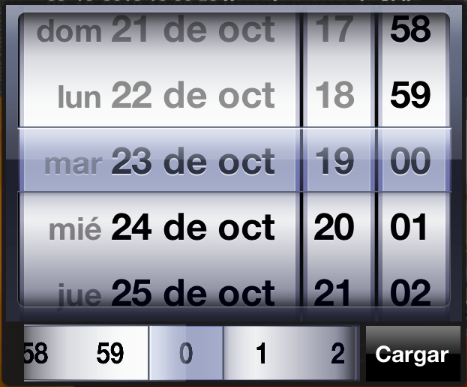
\includegraphics[scale=0.5]{imgs/datepicker-mod.png}
	\caption{Control del tiempo de la transmisión, UIDatePicker y UIPicker modificado}
	\label{datepicker-mod}	
\end{figure}
 
		\subsubsection{UIButton}
		El reproductor presenta botones de control de reproducción en base a un reproductor estándar de MPMoviePlayerViewController, estos son PLAY/PAUSE, Next. Estos botones son lo único que comparten con un reproductor normal ya que además se debe incorporar un botón para compartir el momento de la reproducción a través de redes sociales. Se agrega entonces un botón con el icono de twitter que presenta un formulario de acción con ítems para cerrar la sesión, compartir en twitter o cancelar la acción de compartir.
		
%				play pausa, ibactions
		\subsubsection{Volume Slider}

		Para presentar el control de volumen se utilizó una clase estandar del sistema operativo, llamada MPVolumeslider, encargada de presentar un deslidador que está directamente relacionado con los botones del hardware de los dispositivos iOS. Tanto así, que en materia de debuggeo, el simulador no permite mostrar en pantalla dicho control. Se agrega ajustando un rectangulo destinado como perimetro para que el sistema presente dicho control mediante una subvista.
		
		\subsubsection{Vistas de Tablas}
%		volumen, slider de view controller tipo facebook, etc
Para representar el cliente de twitter se utilizó una instancia de la clase UITableView, clase que tiene como fin presentar y editar listas jerárquicas de información. La infomación se obtiene del resultado de una llamada a twitter utilizando su API de búsqueda. El resultado consiste en un archivo JSON (\textit{JavaScript Object Notation}) que contiene los tweets de los últimos 6 a 9 días respecto a la consulta realizada. Para el caso de esta aplicación, se utiliza el hashtag \textbf{\#SocialStream} como se puede ver en la figura \ref{sshot-twitterclientvc}.\\

Para poder presentar la tabla sin perder parte de la transmisión se muestra el cliente de twitter bajo la vista del reproductor. Utilizando la clase ZUUIRevealController fue posible apilar en pantalla dos controladores de vista: TwitterClientVC y StreamPlayerVC. Para lograr presentar el controlador de vista inferior, fue necesario asociar a la vista del reproductor un botón que permita arrastrar con el dedo o desplazar con un toque la vista que lo posee. Esto se realizó asociando la acción de tocar dentro del botón y el gesto \textit{navigationBarPanGestureRecognizer} a la barra que lo contiene. El método asociado \textit{revealToggle:} de la instancia de ZUUIRevealController permite mostrar, ocultar o arrastrar las vistas superpuestas. En la figura \ref{sshot-twitterclientvc} se muestra el instante donde el usuario arrastra la vista del reproductor a través del botón \textbf{Twitter}.


\begin{figure}[H]
	\centering
	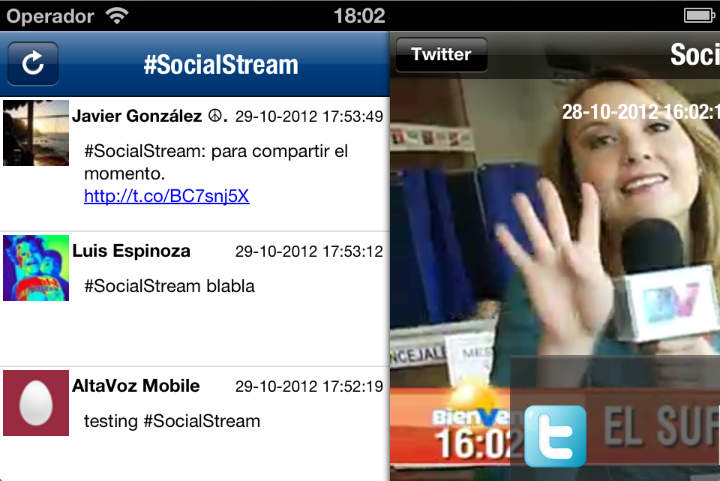
\includegraphics[scale=0.4]{imgs/sshot-twitterclientvc.png}
	\caption{Revelación del cliente de Twitter en base a UITableView}	
	\label{sshot-twitterclientvc}
\end{figure}
 
 
%\clearpage
\section{Integración Redes Sociales}
	%diagrama de como funciona el posteo y recepcion de twitts
	Para destacar la connotación de caracter social de la aplicación, se incorporó un sistema de compartimiento en base a la red social Twitter. Este sistema no se limita solamente a esta red social, es posible incorporar otras, sólo que se utilizó ésta como ejemplo.\\
	
	En resumen, el usuario al pulsar el botón \textbf{\textquotedblleft t\textquotedblright} visible en la imagen \ref{sshot-twitterclientvc} genera un URL en base a la fecha de la transmisión que está viendo, este URL se comprime a través del servicio bit.ly con tal de aminorar la cantidad de caracteres en el mensaje y luego se entrega al usuario en un campo de texto donde se le permite describir lo que comparte. Una vez en la red Twitter, usuarios que observen este mensaje a través de la misma aplicación pueden llegar a reproducir el instante compartido por el autor del mensaje.
	
	
	\subsection{Twitter}
	%http://www.alexa.com/siteinfo/twitter.com
	La red de microblogging Twitter permite difundir mensajes de forma pública y también privada a millones de usuarios en internet, siendo uno los sitios más populares de la web\cite{alexa-twitter} permitiendo que personas no suscritas puedan ver los mensajes.
	La limitante de cada mensaje se reduce a 140 caracteres, más que suficientes para difundir enlaces desde la aplicación desarrollada y permitiendo además una pequeña descripción por parte del usuario.
		\subsubsection{API Twitter}
		Para la muestra de los mensajes compartidos, se utilizó \textit{Twitter Search API}, interfaz dedicada a búsquedas en el índice de mensajes (\textit{tweets}) en tiempo real. Esta se caracteriza por lo siguiente:
		
		\begin{itemize}
		\item Su historial dura no más de una semana, el indice de mensajes abarca entre 6 a 9 días.
		\item La búsqueda no requiere de autenticación, se realiza anonimamente.
		\item El resultado de la búsqueda se basa en relevancia del tema en vez de la totalidad de sus mensajes. Esto debido a las políticas del servicio de Twitter donde se privilegia el alcance de los mensajes según la reputación de los usuarios \cite{twitter-relevance}.
		\end{itemize}

Tomando en cuenta estos puntos Search API satisface la obtención de mensajes compartidos desde la aplicación cliente, si bien existen alternativas dispuestas por twitter para la obtención de mensajes, no significan una mejora respecto al fin de la aplicación cliente. Se prefiere por su simpleza.
		
%		las llamadas de twitter que se utilizarán
		\subsubsection{Sharekit vs. Twitter Framework}
%		el porqué se utilizó sharekit en vez de twitter framework, el argumento de las apps de twitter
Durante el desarrollo de la aplicación cliente Apple Inc. lanzó al público el sistema operativo iOS 5, el cual permite entre muchas caracteristicas, la integración del sistema con la red social Twitter mediante \textbf{Twitter.framework} . Por simpleza y compatibilidad con versiones anteriores de iOS se descartó utilizar esta nueva herramienta para utilizar la biblioteca de código libre \textbf{Sharekit}\cite{library-sharekit}, destinada a integrar todo tipo de redes sociales incluyendo twitter. Otro motivo de esto es la posibilidad de expandir a otras redes el contenido que se comparte a través de la aplicación cliente. \\

En caso que se desee, es posible utilizando Sharekit modificar el mensaje a compartir de forma que el usuario no elimine el URL relacionado al contenido compartido.

		\subsubsection{Post en Twitter}
%		como postear en twitter desde la app, action sheet
		Para entregar el momento que se está viendo u oyendo, es necesario tener la fecha de la transmisión, esto se obtiene de uno de los observadores periódicos encargados de la fecha del flujo de datos (\ref{observer-date}). El objeto obtenido es una instancia de la clase \textbf{NSDate}, encargada de registrar información temporal, convenientemente se utiliza el método de la clase: \textit{\textbf{timeIntervalSince1970}} que entrega la cantidad de segundos entre el 1 de enero de 1970 y la fecha en cuestión, el valor obtenido es del tipo \textbf{\textit{double}} por lo tanto es necesario convertir el valor a NSString, cadena de caracteres.
		
		
		En caso de no tener el valor para la fecha en reproducción la aplicación no permite compartir.

		\subsubsection{Seguimiento de Hashtag}
		%las llamadas de url para el cliente de twitter
		Para realizar el seguimiento de los mensajes se utiló Search API como se explicó anteriormente. Para realizar la llamada se realiza una conexión con el URL: 
\url{http://search.twitter.com/search.json?include_entities=true&q=%23SocialStream} \\
		
		Nótese que el último componente del URL corresponde al hashtag, o marca de seguimiento que se se utiliza en los mensajes. La respuesta por parte de Twitter es un objeto del tipo JSON que contiene un arreglo con los mensajes resultantes.

\begin{figure}[H]
	\centering
	\begin{lstlisting}
"created_at": "Thu, 08 Nov 2012 21:21:59 +0000",
"entities": {
    "hashtags": [
    		{ "indices": [ 0, 13 ], 
    		  "text": "SocialStream" }],
    "urls": [
        { "display_url": "bit.ly/SPCO4a",
            "expanded_url": "http://bit.ly/SPCO4a",
            "indices": [ 30, 50 ],
            "url": "http://t.co/uKm7VRMb" } ],
    "user_mentions": [] 
    },
"from_user": "javiergov",
"from_user_id": 76853723,
"from_user_id_str": "76853723",
"from_user_name": "Javier Gonzalez O.",
"geo": null,
"id": 266651804614418430,
"id_str": "266651804614418432",
"iso_language_code": "en",
"metadata": { "result_type": "recent" },
"profile_image_url": "http://url.del.avatar/foto.jpg",
"source": "&lt;a href=&quot;http://sitio.dela.app&quot;
					&gt;SocialStream for iOS&lt;/a&gt;",
"text": 
"#SocialStream http://t.co/uKm7VRMb texto del tweet",
"to_user_id": 0,
"to_user_id_str": "0",
        	\end{lstlisting}
	\caption{Componentes de un Tweet, respuesta de Twitter Search API}
	\label{tweet-json}	
\end{figure}			

		
		\subsubsection{Extracción de información de un Tweet}
%		como se parseó el json con los twitts y saber si eran sstream
Para presentar los mensajes de forma simple para el usuario fue necesario serializar el objeto JSON obtenido de Seach API. Gracias al componente \textbf{NSJSONSerialization} del entorno de desarrollo de iOS, como se muestra en \ref{json-serialization}, es posible generar un objeto del tipo NSDictionary para ser entregada a la clase encargada de generar la tabla con los mensajes.

\begin{figure}[H]
	\centering
\begin{lstlisting}
NSError *error = nil;
NSDictionary *dict =
[NSJSONSerialization 
		JSONObjectWithData:responseData 
				   options:NSJSONReadingMutableLeaves
                   	 error:&error];
if (error) 
 MLogString(@"serialization error: %@",
 					[error description]);
\end{lstlisting}
	\caption{Obtención de los datos desde JSON mediante NSJSONSerialization}
	\label{json-serialization}
\end{figure}	

Una instancia de NSDictionary posee una cadena de claves y valores asociados, la generada del objeto JSON entrega valores de las claves encontradas en la figura \ref{tweet-json}.
Para presentar el contenido en la tabla de la interfaz gráfica se utilizaron los valores de las claves:
\begin{itemize}
\item \textbf{\textquotedblleft from\_user\_name"}: (línea 16) El nombre completo del usuario.
\item \textbf{\textquotedblleft text"}: (línea 25) El cuerpo del mensaje.
\item \textbf{\textquotedblleft profile\_image\_url"}: (línea 22) La dirección a la imagen que el usuario utiliza como avatar.
\item \textbf{\textquotedblleft created\_at"}: (línea 1) La fecha en que se realizó el tweet, tomar en cuenta que no corresponde a la fecha de la transmisión que el usuario comparte. 
\end{itemize}
Al pulsar en algún mensaje representado en la tabla \ref{sshot-twitterclientvc}, se utiliza el valor de la clave \textit{\textbf{\textquotedblleft expanded\_url"}} (\ref{tweet-json}, línea 8) para analizar si su contenido es utilizable por la aplicación.

	\subsection{Bit.ly}
%		desmenuzar el enlace de bitly
Para entregar una buena experiencia al usuario se utilizó el servicio de compresión de URL \textbf{Bit.ly}, de forma que el enlace al stream (que además incluye marca de tiempo) no utilice demasiados caracteres. El motivo es la limitante de twitter de 140 caracteres por mensaje, los cuales la aplicación debe utilizar lo mínimo para compartir.\\

Otra característica útil para la supervisión de la aplicación y el servicio \textit{SocialStream} en su totalidad, es la posibilidad de utilizar las llamadas a la API de Bit.ly junto a las credenciales de una cuenta previamente hecha para llevar un registro del uso de los enlaces. \\

La compresión se debe realizar al compartir en twitter un enlace al stream, y descompresión cuando el usuario pulsa en un tweet de la tabla (figura \ref{sshot-twitterclientvc}).

		\subsubsection{API Bit.ly}
%		las llamadas de la api que se utilizaron
%		http://dev.bitly.com/api.html

Para utilizar y mantener el registro de los enlaces compartidos, se configuran credenciales obtenidas del sitio web \cite{bitly-settings} (nombre de usuario y Legacy API Key) en un archivo de cabecera de la biblioteca Sharekit.


		
		\subsubsection{Compresión de URL}
Para comprimir un URL se realiza una petición al servidor con el comando \textit{\textbf{shorten}} utilizando el URL que se muestra en la figura \ref{bitly-shorten} y con argumentos en la cadena de consulta para los campos: login, apikey, longUrl y format.

\begin{figure}[H]
	\centering
\begin{lstlisting}
http://api.bit.ly/v3/shorten?
					login=usuario
					&apikey=R_1234567890
					&longUrl=http%3A%2F%2Fgoogle.com%2F
					&format=txt
\end{lstlisting}
	\caption{Ejemplo de URL para compresión con Bit.ly API}
	\label{bitly-shorten}
\end{figure}	

La respuesta entregada depende del campo \textit{format} especificado en la cadena de consulta. En el ejemplo de la figura \ref{bitly-shorten} se espera en formato de texto plano, en caso de no definir formato la respuesta se entrega como objeto JSON.\\

Para una respuesta exitosa se recibe una cadena de caracteres con el URL comprimido de tipo 
\textbf{http://bit.ly/\textless hash comprimido\textgreater} \\

En caso de cualquier falla, el texto entregado es la causal misma del error, por lo tanto cual sea la respuesta debe ser analizada su integridad como URL antes de ser entregada al resto de las instancias de las clases que componen la aplicación. Esta comprobación se realiza comparando el \textit{scheme} del \textbf{NSURL} creado a partir del texto resultante, en caso de ser \textbf{http} o \textbf{https} se considera conforme por parte de la aplicación.\\ 

Algunas respuestas erroneas pueden ser:
\begin{itemize}
\item INVALID\_APIKEY: Clave para acceder a la API es inválida o no concuerda con el usuario. 
\item INVALID\_LOGIN: El nombre de usuario no corresponde a la clave de API o no existe.
\item INVALID\_ARG\_FORMAT: El formato requerido no corresponde a los dispuestos a entregar por Bit.ly, los cuales son txt, json o xml.
\item INVALID\_URI: El recurso a comprimir no se entrega codificado en código porciento\cite{percent-encoding}.
\end{itemize}

		\subsubsection{Expansión de atajo bit.ly}
%		como se expande un url de bitly y se usa en la app
Para expandir un URL comprimido por Bit.ly se utiliza la llamada a la API de forma similar al método de compresión, se diferencia con el comando \textit{\textbf{expand}} en vez de \textit{shorten} y entregando el hash comprimido del enlace corto obtenido del valor de la clave \textit{\textbf{\textquotedblleft expanded\_url"}} includo en un tweet (\ref{tweet-json}, línea 8). El hash comprimido corresponde a la ruta del URL.

\begin{figure}[H]
	\centering
\begin{lstlisting}
http://api.bit.ly/v3/expand?
						login=usuario
						&apikey=R_1234567890
						&hash=WQfFTO
\end{lstlisting}
	\caption{Ejemplo de URL para expandir hash comprimido perteneciente a un URL Bit.ly}
	\label{bitly-expand}
\end{figure}	
Nótese que en el URL de la figura \ref{bitly-expand} no especifica formato de respuesta, por lo tanto se recibe por defecto un objeto JSON. El motivo de este cambio es sólo de investigación, ya que de esta forma se puede obtener mayor información que una respuesta de sólo texto.

\begin{figure}[H]
	\centering
\begin{lstlisting}
{   "data": {
        "expand": [
            { 	"global_hash": "900913",
                "hash": "WQfFTO",
                "long_url": "http://google.com/",
                "user_hash": "WQfFTO" }]},
    "status_code": 200,
    "status_txt": "OK" }
\end{lstlisting}
	\caption{Respuesta exitosa de tipo JSON al expandir URL Bit.ly}
	\label{bitly-json-response}
\end{figure}	
Los datos del resultado de la llamada se entregan a una instancia de NSJSONSerialization con el mismo método utilizado para desmenuzar la información de los tweets (fig. \ref{json-serialization}). De esta forma se obtiene un objeto del tipo NSDictionary y para luego facilmente obtener el valor asociado a la clave \textbf{\textquotedblleft long\_url"}.
En caso de obtener como respuesta un error los datos serán de igual forma del tipo JSON, sólo que la información de la clave \textbf{\textquotedblleft status\_txt"} correspondrá a la causa del error en vez del OK que se obtiene al realizar una operación exitosa (fig. \ref{bitly-json-response}). El valor de las causas de error son las mismas que las indicadas anteriormente.

%NOT_FOUND
		\subsubsection{Seguimiento de un Hipervínculo}		
%		como se monitorean los twitts por bitly y se puede usar pa marketing, saber que es lo popular etc		
El hecho de entregar las credenciales de una cuenta al comprimir y expandir URL con Bit.ly permite monitorear los enlaces compartidos y la cantidad de aperturas que estos tienen. Esta información puede ser de gran ayuda para identificar qué programas o secciones transmitidas en la señal son más populares, de forma similar a lo que es el \textit{\textquotedblleft people meter"} o rating en la televisión abierta.

Esta información se encuentra en \textbf{\url{https://bitly.com/a/stats}} donde es necesario acceder con las mismas credenciales configuradas en la aplicación.

\clearpage
\section{Registro en iOS}
El sistema operativo iOS permite registrar \textit{schemes}, con lo cual el sistema reconoce qué aplicación debe encargarse de interpretar cierto URL. Esta característica es aprovechada por la aplicación cliente de forma que los enlaces compartidos por los usuarios en Twitter lleven a la aplicación cliente sin que esté necesariamente en ejecución.
	\subsection{Schemes}
%	explicar que son los schemes
	Un \textbf{\textit{Scheme}} es el prefijo de un \textit{Universal Resource Locator} (\textbf{URL}), el cual define el protocolo a utilizar para ubicar un recurso.
	Es necesario además que se pueda acceder al contenido compartido a través de la Web o incluso desde otras aplicaciones del sistema.

Para esto es necesario que la aplicación indique en su archivo de información general \textbf{\textquotedblleft info.plist\textquotedblright}  \ los schemes de los URL que tiene interés.
En el caso de la aplicación cliente, se registra un scheme como \textquotedblleft socialstream\textquotedblright , de manera que URLS de la forma \textbf{\url{socialstream://www.ejemplo.com/}} sean entregados a la aplicación cliente.

% http://developer.apple.com/library/ios/documentation/iPhone/Conceptual/iPhoneOSProgrammingGuide/AdvancedAppTricks/AdvancedAppTricks.html#//apple_ref/doc/uid/TP40007072-CH7-SW50

	\subsection{Redireccionamiento via Web}
%	explicar breve como funcionará la carga del scheme sstream, en web y mobile
La forma más simple que se ideó para entregar la información, según las variadas plataformas que se conectan a internet, consiste en comunicar a través de la herramienta común que poseen los móviles y computadores: el navegador web.\\

El navegador web al iniciar la conexión través del protocolo HTTP con cierta página remota entrega dentro de sus cabeceras el Agente de Usuario \textit{(user agent)}, con lo cual es posible identificar qué cliente se conecta y a la vez personalizar el contenido a entregarle.

		\subsubsection{PHP Script}
		\label{subsec:php-redir}
%		explicar brevemente el script php 
Se desarrolló un script en PHP, encargado de identificar el cliente que se está conectando al servidor y según el tipo de dispositivo o navegador redirecciona a un URL con scheme personalizado, o presenta una página web con información a social stream.\\

El acceso al script requiere, para su buen funcionamiento, ciertos campos como mínimo relacionados con la transmisión que se compartió y se incluyen en el URL, como query strings (cadena de consulta), estos son el tipo de canal y la marca de tiempo, similares a los entregados al dispatcher por parte del cliente se hace una petición de lista de reproducción.
El script se encarga de analizar las marcas de tiempo y tipo de señal para entregar un URL especial según el agente de usuario del cliente que hace la petición.\\

El agente de usuario se identifica llamando la función PHP \textbf{\$\_SERVER['HTTP\_USER\_AGENT']} y a través de expresiones regulares fue posible diferenciar cada tipo de cliente.

		\subsubsection{Respuestas según User Agent}
%		describir los casos según user agents
\textbf{Apple Device}: En caso que el cliente que hace una petición al script en el servidor sea un dispositivo movil Apple, entiendase iPod, iPhone o iPad, se genera un URL especial con el scheme registrado por la aplicación en el sistema operativo iOS, en el caso de este proyecto \textquotedblleft socialstream\textquotedblright . Este URL se entrega al cliente como redirección, teniendo como metodo de respaldo en caso que el cliente no tenga instalada una aplicación que maneje este scheme, un redireccionamiento al sitio de descarga de la aplicación en iTunes Store, utilizando el scheme "itms" que es manejado por el sistema para efectos de descarga de aplicaciones. \\ 

Tomando en consideración que este proyecto es un desarrollo experimental que no se ha llevado a producción, la redirección en la tienda oficial de Apple lleva a otra aplicación desarrollada y lanzada por el alumno en: \url{itms://itunes.apple.com/cl/app/df-mercados/id483602458?mt=8\&uo=6} \\

Esta redirección sólo tiene motivos de prueba, para simular el método de difusión de aplicaciones al compartir contenido socialmente.
El agente de usuario que entregan los dispositivos Apple tienen como formato: 
	\begin {lstlisting}
Mozilla/5.0 (iPhone; CPU iPhone OS 5_1 like Mac OS X) 
AppleWebKit/534.46 (KHTML, like Gecko) 
Version/5.1 Mobile/9B179 Safari/7534.48.3
Apple Device - Mobile Safari.
\end{lstlisting} 
~\\ % para forzar una nueva linea \newline ni \*[espacio] funcionan

\textbf{Android}: En el caso de Android, a la fecha del desarrollo de la aplicación cliente, la versión del sistema operativo con mayor adopción por los usuarios es Gingerbread (2.3.x), debido a que Ice Cream Sandwich (4.0.x) aun se encontraba en desarrollo y prueba. Considerando que Gingerbread no es compatible con el protocolo HTTP Live Streaming y para nuevas versiones la compatibilidad se encuentra en desarrollo, se da aviso al navegador web que accede al servidor con el mensaje \textquotedblleft Android no es compatible con HTTP Live Streaming".\\

\textbf{Navegadores Web}:
Para navegadores con la marca HTML5 \textless video\textgreater \ incompatible con HTTP Live Streaming como por ejemplo Firefox y Opera, se da aviso presentando una página web con el mensaje: \textquotedblleft Tu navegador no es compatible con HTTP Live Streaming". \\

En el caso del navegadores que utilizan el motor de renderizado Webkit como Chrome y Safari, se debe diferenciar la compatibilidad con el protocolo HLS, ya que Safari es capaz de mostrar el contenido. Para Chrome se presenta una página web similar al caso de Opera y Firefox, sin embargo para Safari se presenta una página especial con un reproductor generado con la marca \textless video\textgreater , donde la fuente del stream es el URL de la lista de reproducción que se entrega a la aplicación cliente cuando hace una petición de cambio temporal. Como Safari es capaz de reproducir streams HLS es posible ver sólo flujo compartido, no es posible compartir ni controlar el flujo de la transmisión a menos que se desarrolle una aplicación web que se comporte de forma similar al cliente iOS.\\

El reproductor recibe como entrada una lista de reproducción generada por el \textit{playlist dispatcher} con los parámetros compartidos en la cadena de consulta \textbf{s} y \textbf{t}.



		
		